\section{Volba barevné palety aplikace}\label{draft:colors}

Barvy použité v aplikaci mají velký vliv na to, jak ji budou její uživatelé vnímat. Důležitý je jak kontrast barvy textu a pozadí, tak i volba barev akčních či informativních prvků.

\paragraph{Kontrast barvy textu a barvy pozadí.} Základem pro čitelnost textu je správný kontrast barvy textu a barvy pozadí, na kterém se text nachází. Například klasický černý (\#000000) text na bílém (\#FFFFFF) pozadí má kontrastní poměr 21:1, což je nejvyšší možný. Konsorcium W3 vydalo dokument \cite{w3-access-guide}, který popisuje, jak by měl vypadat správně dostupný web - jedna sekce popisuje právě i kontrast. Uvedu úryvek z dokumentu:
\begin{itemize}
    \item \emph{Kontrast (minimum)}: Vizuální prezentace musí mít minimální kontrastní poměr 4,5:1, s následujícími výjimkami:
    \begin{itemize}
        \item \emph{Velký text}: Musí mít kontrastní poměr minimálně 3:1.
        \item \emph{Dekorativní, skryté a doprovodné prvky a logotypy}: Bez požadavků na minimální kontrastní poměr
    \end{itemize}
    \item \emph{Kontrast (pokročilý)}: Vizuální prezentace by měla mít minimální kontrastní poměr 7:1, s následujícími výjimkami:
    \begin{itemize}
        \item \emph{Velký text}: Měl by mít kontrastní poměr minimálně 4,5:1.
        \item \emph{Dekorativní, skryté a doprovodné prvky a logotypy}: Bez požadavků na minimální kontrastní poměr
    \end{itemize}
\end{itemize}

Zde samozřejmě platí, že čím více chceme text na stránce zdůraznit, tím větší kontrastní poměr mu dáme.

\paragraph{Volba barev akčních a informačních prvků.} U informačních prvků je zde poměrně klasické rozdělení: zelená jako potvrzovací, modrá - informativní, žlutá - varovná a červená - chybová. Pro akční tlačítka pak typicky zelená - vytvoření, modrá - zobrazení, žlutá - úprava a červená - smazání. V aplikaci ale většinou nechceme mít tolik barev, moderní aplikace mají čistší, jednodušší design, který když je proveden správně, může snížit zátěž uživatele a zvýšit přehlednost. Velmi často se dnes objevují definice barev jako \code{primary}, \code{secondary} (občas i \code{tertiary}) a \code{accent}, které se jednou zvolí a poté se napříč aplikací používají vlastně jako proměnné.

Výběrem těchto tří barev se zabývá mnoho článků a stránek. Teorie, na které ale všichni staví, je pořád stejná: Když volíme tři barvy, existují tři nejčastěji používaná barevná rozložení \cite{color-scheme-pick}:

\begin{enumerate}
    \item \emph{Trojúhelníková}: Rovnoměřné rozdělení barev přes celé barevné schema. Jedná se o velmi výrazné schema, a to i v případě použití nižší barevné saturace. Ideální použití je jedna základní barva a dvě akcentní.
    \begin{figure}[h]
        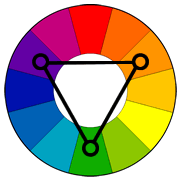
\includegraphics[width=0.2\textwidth]{../png/colors/Triad.png}
        \caption{Barevná paleta aplikace: Trojúhelníkové schema} \label{picture:colors:analog}
    \end{figure}
    \item \emph{Rozděleně-doplňková}: Toto schema vychází z doplňku dvou barev, tedy barev, které jsou v paletě naproti sobě, protější barva je ale rozdělena na dvě. Oproti trojúhelníkovému schematu je méně výrazné, díky čemuž je jednodušší barvy zvolit tak, aby nebyly pro uživatele příliš útočné. Ideální použití je opět jedna základní barva a dvě akcentní.
    \begin{figure}[h]
        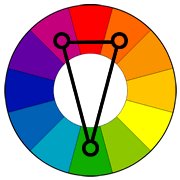
\includegraphics[width=0.2\textwidth]{../png/colors/SplitComplementary.png}
        \caption{Barevná paleta aplikace: Rozděleně-doplňkové schema} \label{picture:colors:splitCom}
    \end{figure}
    \item \emph{Analogová}: Zvolené barvy jsou v barevné paletě přímí sousedé a jedná se tak o \uv{klidné} rozložení, které vytváří jemný design, jenž je často vidět i v přírodě. Problémem zde může být vhodná volba kontrastu, protože barvy nejsou samy vůči sobě příliš kontrastní a je nutné je od sebe alespoň trochu rozlišit. Ideální použití je jedna dominující barva, druhá doplňková a třetí jako akcentní.
    \begin{figure}[H]
        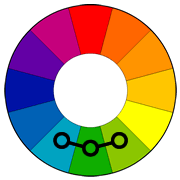
\includegraphics[width=0.2\textwidth]{../png/colors/Analogous.png}
        \caption{Barevná paleta aplikace: Analogové schema} \label{picture:colors:triad}
    \end{figure}
\end{enumerate}

\paragraph{Volba barev pro mou aplikaci.} Jelikož cílem aplikace je pomáhat při práci ve skladu a upozorňovat na důležité zprávy, vyloučil jsem hned ze začátku \emph{analogové} barevné schema, protože jeho barevné rozložení patří spíše na stránky, které jsou pasivnější, nevyžadují tolik interakce s uživatelem a spíše obsah prezentují, než aby vyžadovaly jeho zadávání. Zbyla mi tedy velmi podobná rozložení \emph{trojúhelníkové} a \emph{rozděleně-doplňkové}. Podle osobního pocitu jsem vybral základní klidnou barvu: šedozelenou \#009688, a k ní doplňkově-akcentní růžovou \#E91A63 a čistě akcentní tmavě žlutou \#FFC107, jejichž rozložení na barevné paletě je vidět na obrázku \ref{picture:colors:app}. Společně tyto barvy tvoří něco mezi dvěma zvolenými schematy - trojůhelník není ani pravidelný, ani se neblíží k doplňku.\\

\begin{figure}[h]
    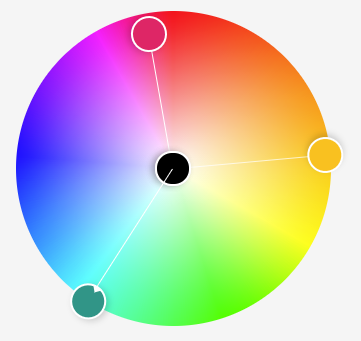
\includegraphics[width=0.35\textwidth]{../png/colors/app.png}
    \caption{Barevná paleta aplikace: Zvolené schema pro mou aplikaci} \label{picture:colors:app}
\end{figure}

\paragraph{Barvy a idempotence akce.} Jelikož mám vybrané dvě akcentní barvy, musel jsem se rohodnout, kde budu kterou z nich používat. Co se týká zobrazování, je vše poměrně jasné: k základní barvě se volně váže doplňkově-akcentní růžová, a čistě akcentní žlutá barva je ponechána pouze pro důležité položky, které je potřeba speciálně zvýraznit. Jiné je to ale u akcí - tlačítek, odkazů apod. Zde jsem se rozhodl barvu tlačítek volit dle idempotence akce, kterou vyvolávají - tedy zda vyvolaná akce způsobuje vedlejší efekty, nebo ji lze vyvolávat stále dokola. Za vedlejší efekty v aplikaci považuji následující situace:
\begin{itemize}
    \item navigace na jinou stránku,
    \item uložení či úprava dat.
\end{itemize}
Naopak akce, které nemají vedlejší efekt, jsou všechny ty, které neukládají žádná data ani nemění navigaci, mohou ale měnit aktuální zobrazení stránky, tedy například něco otevřít, skrýt, přesunout, avšak vždy tak, že se jedná o akci pouze na jednom klientu a zůstávají na jedné stránce. Na obrázcích \ref{picture:colors:time_tracker} a \ref{picture:colors:task_fab} je vidět použití jak idempotentních, tak non-idempotentních akcí: tlačítka \emph{storno} a hlavní akční tlačítko pouze skrývají dialog, respektive rozevírají menu, kdežto ostatních tlačítka a volby vždy buďto odesílají data, nebo přecházejí na novou stránku.

\begin{figure}[]
    
\includegraphics[width=0.6\textwidth]{../png/app/colors_time_tracker.png}
    \caption{Barvy znázorňující idempotenci akcí: Dialog běžícího času} \label{picture:colors:time_tracker}
\end{figure}
\begin{figure}[]
    
\includegraphics[width=0.3\textwidth]{../png/app/colors_tasks.png}
    \caption{Barvy znázorňující idempotenci akcí: Tlačítko tvorby úkolu} \label{picture:colors:task_fab}
\end{figure}
